% Presentation: JMM - Alexander and Cooper
% Date: Saturday January 7, 2023
\documentclass[10pt]{beamer} %document class
\usetheme{default} %theme
% load packages

\usepackage[utf8]{inputenc}
\usepackage{framed,color}
\usepackage{amsmath}
\usepackage{soul}
\usepackage{geometry}
\usepackage{fancyhdr}
\renewcommand{\headrulewidth}{0pt}
\usepackage{graphicx}
\usepackage{float}
\usepackage{tikz}
\usetikzlibrary{calc,matrix,positioning}
\usepackage{wasysym}
\usepackage{xcolor}
\usetikzlibrary{calc,arrows,positioning,shapes,shapes.gates.logic.US,trees}
\usepackage{mathtools}
\usepackage{multirow}
\usepackage{color}
\usepackage{xcolor}
\usepackage{lipsum}
\usepackage{soul}
\usepackage{tabularx}
\usepackage{titling}

%%% ENV FOR DEF
\usepackage{amsthm}\setbeamertemplate{theorems}[numbered] % to number

\theoremstyle{plain} % insert bellow all blocks you want in italic
%\newtheorem{theorem}{Theorem}[section] % to number according to section

\theoremstyle{definition} % insert bellow all blocks you want in normal text
%\newtheorem{definition}{Definition}[section] % to number according to section
\newtheorem*{idea}{Proof idea} % no numbered block

\usepackage{graphicx}
\usepackage{tcolorbox}

\usepackage[labelfont=bf]{caption}
\captionsetup[figure]{labelfont={bf},name={Figure},labelsep=period}



% settings
\setlength{\arrayrulewidth}{0.5mm}
\setlength{\tabcolsep}{18pt}
\renewcommand{\arraystretch}{1.5}

% defining the color marron to change the remove text included in the slide theme
\definecolor{Maroon}{cmyk}{0, 0.87, 0.68, 0.32}

% section structure
\AtBeginSection[]{
  \begin{frame}
  \vfill
  \centering
  \begin{beamercolorbox}[sep=8pt,center,shadow=true,rounded=true]{title}
    \usebeamerfont{title}\insertsectionhead\par%
  \end{beamercolorbox}
  \vfill
  \end{frame}
}

% title slide
\title{\Large \color{Maroon} Toward a Critical Analysis of \\ Cooperative and Non-Cooperative Games}
\subtitle{\scriptsize \color{Maroon} \sc }
% authors
\author{\tiny Nathan Alexander, PhD \\ Assistant Professor \\ Department of Mathematics \\ Morehouse College \\ \vspace{.4cm} Jalil Cooper \\ Sophomore \\ Stanford University}
% event
\institute{\tiny \sc 2023 Joint Math Meetings \\ NAM-SIAM Special Session on Quantitative Justice 
}
% remove date
\date{}

% quant histories workshop image logo
%\titlegraphic{\includegraphics[width=2.5cm]{MorehouseLogo.png} }
%\logo{\includegraphics[width=.5cm]{5cube.png}}

%\setbeamertemplate{background} 
%{  \includegraphics[width=#cm,height=#cm]{file-name.jpg}}


\begin{document}

% print title page on the first slide
\begin{frame}
\titlepage
\end{frame}


\begin{frame}{\color{Maroon} Overview of Talk}
Background 
\vfill
Concepts
\vfill
Quantitative matter and methods
\vfill
Conclusions and next steps \\
% mathematical models in the sociological imagination
\vfill
\end{frame}

%% Section I
\section{\color{Maroon} Background}
% use this slide to provide a very brief overview (less than 30 seconds) of the content that will be shared



%%%%% OVERVIEW OF QUANT HISTORIES

\begin{frame}{\color{Maroon} \small Using Critical Frameworks to Explore Mathematics and Its Applications}
%%% IMPORTANT COMMENT: emphasize here that one of the primary goals of our work is to question the very foundations of thinking in mathematical modeling, and to examine a root requirement of critical quantification that requires we begin at and question the very foundational points and narratives

{\color{Maroon} The \textbf{Quantitative Histories Workshop} at Morehouse College} \\ 
\noindent \small Our work engages historical and social content to explore the information that is derived from quantification, its usage, various methods, and interpretations. \\
\vfill
Our lab leads with historical case studies on issues of inequity and injustice to subsequently explore underlying quantitative relations and methods. We seek to confront often emotional and tough historical content prior to quantification. \\
\vfill
We define what is meant by ``critical" within the context of each project. \\
\vfill
\noindent Two sample projects: \\
\vfill
\underline{Beyond the Social in Justice}. This project considers how the continued culmination of quantitative information and evidence of racial injustice in the U.S. might advance us toward material outcomes (e.g., the questions on land in Native and Indigenous communities, reparations for African Americans). 
\vfill
 \underline{Race and the Evolution of Trust} (a working title). This project examines how race-based laws in the U.S. (especially in the late 1800s and early 1900s) and subsequent public policies impacted notions of trust, conflict, and cooperation.
 \vfill
\end{frame}


%%%% RESEARCH PROCESS muliple duplicate slides
\begin{frame}{\color{Maroon} \small Quant Histories Workshop Research Process}
Overall, our research processes are fairly ordered but also nonlinear.
\vfill
\begin{enumerate}
\item Identification and exploration of an historical case or event
\end{enumerate}
\vfill
\end{frame}

%%%% RESEARCH PROCESS
\begin{frame}{\color{Maroon} \small Quant Histories Workshop Research Process}
Overall, our research processes are fairly ordered but also nonlinear.
\vfill
\begin{enumerate}
\item Identification and exploration of an historical case or event
\item Understanding historical context
\end{enumerate}
\vfill
\end{frame}

%%%% RESEARCH PROCESS
\begin{frame}{\color{Maroon} \small Quant Histories Workshop Research Process}
Overall, our research processes are fairly ordered but also nonlinear.
\vfill
\begin{enumerate}
\item Identification and exploration of an historical case or event
\item Understanding historical context
\item Mapping of core concepts
\end{enumerate}
\vfill
\end{frame}

%%%% RESEARCH PROCESS
\begin{frame}{\color{Maroon} \small Quant Histories Workshop Research Process}
Overall, our research processes are fairly ordered but also nonlinear.
\vfill
\begin{enumerate}
\item Identification and exploration of an historical case or event
\item Understanding historical context
\item Mapping of core concepts
\item Understanding historical event(s)
\end{enumerate}
\vfill
\end{frame}

%%%% RESEARCH PROCESS
\begin{frame}{\color{Maroon} \small Quant Histories Workshop Research Process}
Overall, our research processes are fairly ordered but also nonlinear.
\vfill
\begin{enumerate}
\item Identification and exploration of an historical case or event
\item Understanding historical context
\item Mapping of core concepts
\item Understanding historical event(s)
\item Modeling and simulations (if applicable)
\end{enumerate}
\vfill
\end{frame}

%%%% RESEARCH PROCESS
\begin{frame}{\color{Maroon} \small Quant Histories Workshop Research Process}
Overall, our research processes are fairly ordered but also nonlinear.
\vfill
\begin{enumerate}
\item Identification and exploration of an historical case or event
\item Understanding historical context
\item Mapping of core concepts
\item Understanding historical event(s)
\item Modeling and simulations (if applicable)
\item Preliminary outputs and implications
\end{enumerate}
\vfill
\end{frame}

\begin{frame}{\color{Maroon} \small Quant Histories Workshop Research Process}
Overall, our research processes are fairly ordered but also nonlinear.
\vfill
\begin{enumerate}
\item Identification and exploration of an historical case or event
\item Understanding historical context
\item Mapping of core concepts
\item Understanding historical event(s)
\item Modeling and simulations (if applicable)
\item Preliminary outputs and implications
\item Further study
\end{enumerate}
\vfill
\end{frame}


%%%%%% FOCUS OF DISCSUSION
\begin{frame}{\color{Maroon} \small Using Critical Frameworks to Explore Mathematics and Its Applications}
%%% IMPORTANT COMMENT: emphasize here that one of the primary goals of our work is to question the very foundations of thinking in mathematical modeling, and to examine a root requirement of critical quantification that requires we begin at and question the very foundational points and narratives

{\color{Maroon} The \textbf{Quantitative Histories Workshop} at Morehouse College} \\ 
\noindent \small Our work engages historical and social content to explore the information that is derived from quantification, its usage, various methods, and interpretations. \\
\vfill
Our lab leads with historical case studies on issues of inequity and injustice to subsequently explore underlying quantitative relations and methods. We seek to confront often emotional and tough historical content prior to quantification. \\
\vfill
We define what is meant by ``critical" within the context of each project. \\
\vfill
\noindent Two sample projects: \\
\vfill
\underline{Beyond the Social in Justice}. This project considers how the continued culmination of quantitative information and evidences of racial injustices in the U.S. might advance us toward material outcomes (e.g., the questions on land in Native and Indigenous communities, reparations for African Americans). 
\vfill
%% I'd like to highlight this instead of it being blue
\noindent\fcolorbox{yellow}{yellow}{%
    \minipage[t]{\dimexpr1.0\linewidth-2\fboxsep-2\fboxrule\relax}
{ \color{blue} \underline{Race and the Evolution of Trust} (a working title). This project examines how race-based laws in the U.S. (especially in the late 1800s and early 1900s) and subsequent public policies impacted notions of trust, conflict, and cooperation. }
 \endminipage}\hfill
 \vfill
\end{frame}

\begin{frame}{Evolution of Trust interface, designed by Nicky Case}

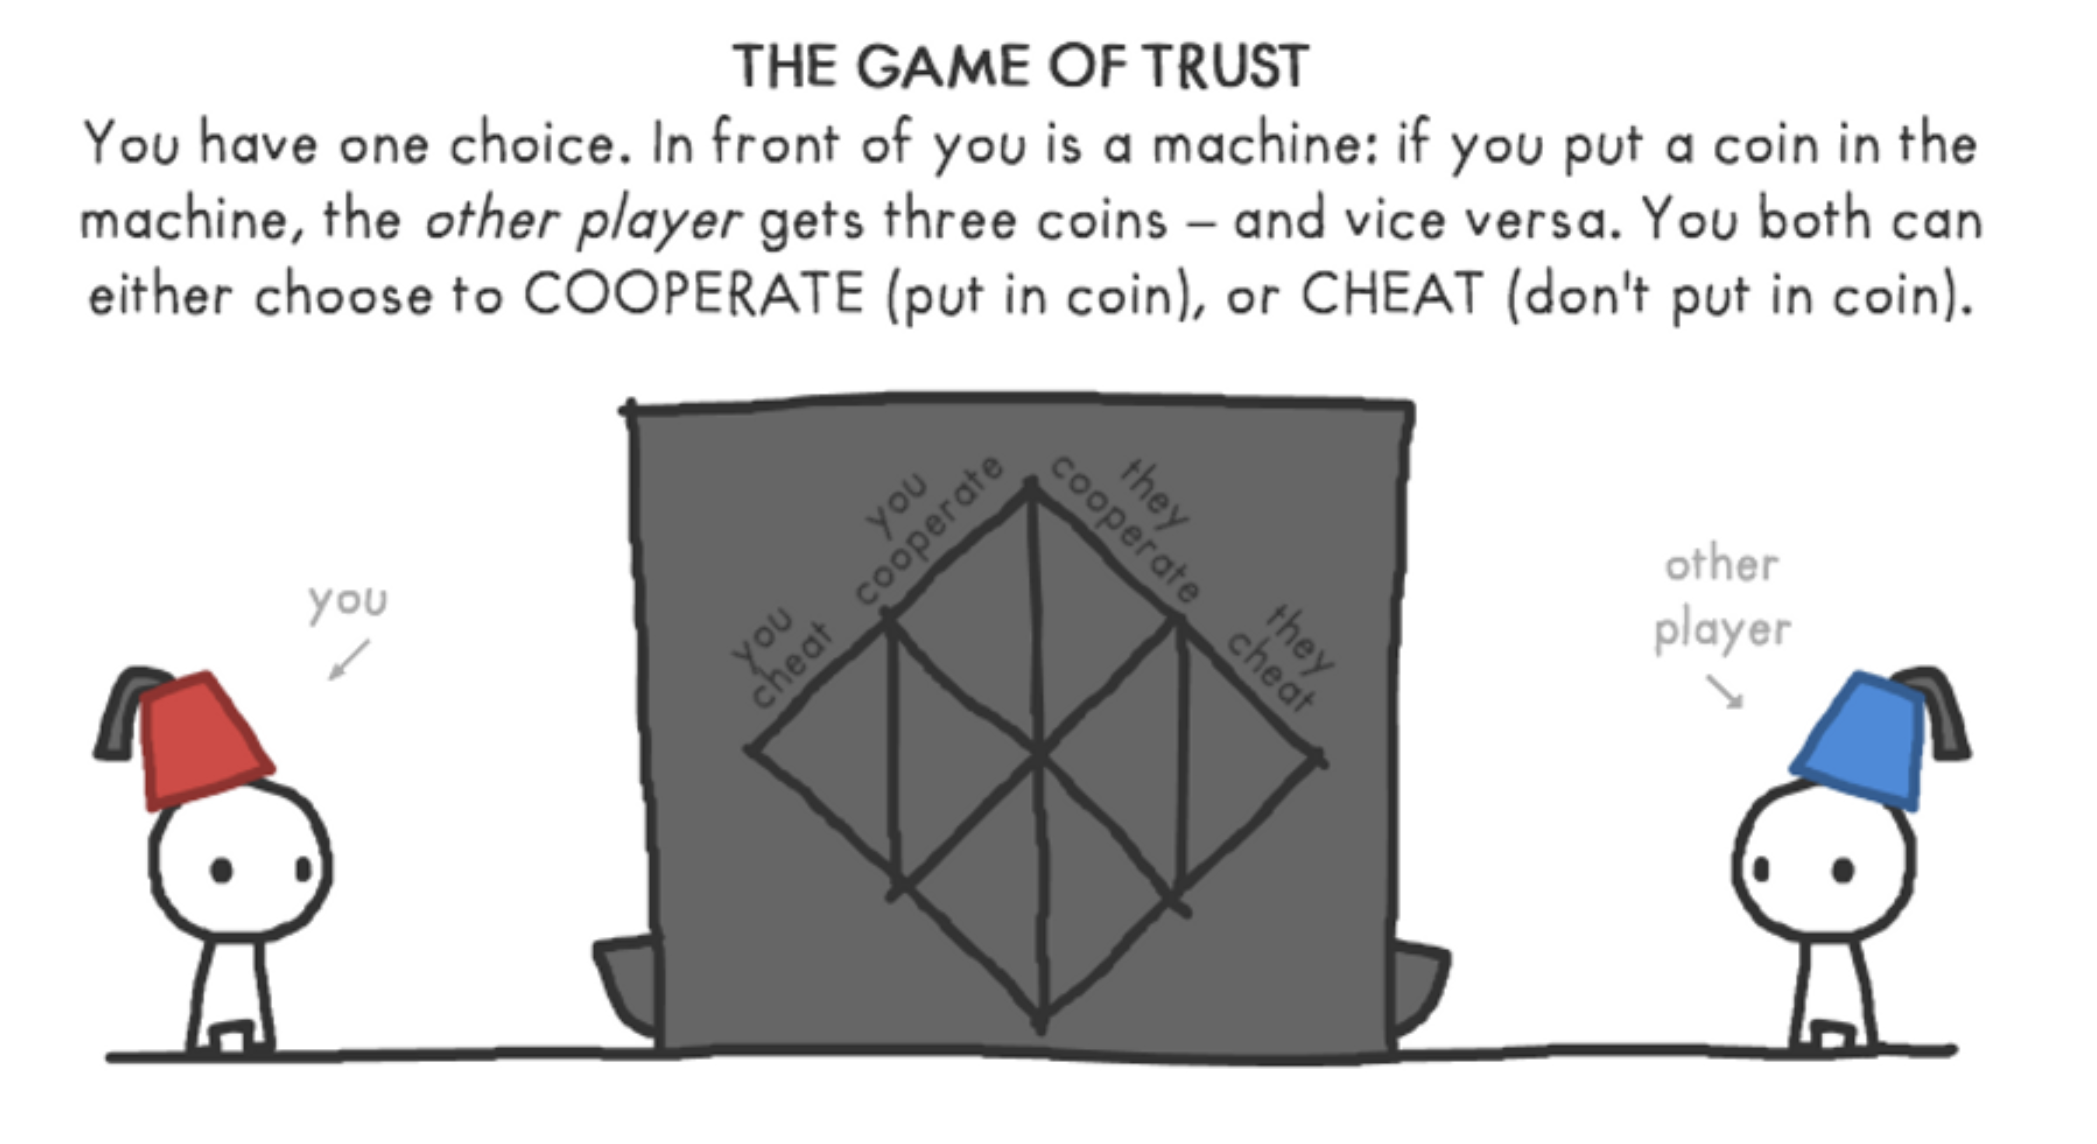
\includegraphics[width=\linewidth]{evolution.png}
\end{frame}

\begin{frame}{\color{Maroon} \small Your Turn!}
Turn to the person next to you to play 3 rounds of the Evolution of Trust Game. \\
\vfill
\noindent Divide your paper into three sections, each section is a round where you have the choice to cooperate or cheat. \\
\noindent After my countdown, you must show the other player your strategy to determine payoffs. Keep track of your final score \\
\vfill
\noindent Payoffs:
\begin{itemize}
    \item Mutual Cooperation: +2 to each player
    \item Cooperation-Cheat: -1 to cooperator. +3 to cheater
    \item Mutual Defection: 0 to each player
\end{itemize}

\end{frame}


\begin{frame}{\color{Maroon} \small Your Turn!}
Turn to the person next to you to play 3 rounds of the Evolution of Trust Game. \\
\vfill
\noindent Divide your paper into three sections, each section is a round where you have the choice to cooperate or cheat. \\
\noindent After my countdown, you must show the other player your strategy to determine payoffs. Keep track of your final score \\
\vfill
\noindent Payoffs:
\begin{itemize}
    \item Mutual Cooperation: +2 to each player
    \item Cooperation-Cheat: -1 to cooperator. +3 to cheater
    \item Mutual Defection: 0 to each player
\end{itemize}
\vfill
\noindent Character profiles of interest: \\
\begin{itemize}
    \item Always Cheat
    \item Always Cooperate
    \item Grudger
\end{itemize}

\end{frame}

\begin{frame}{\color{Maroon} Assumptions and framing}


\begin{tcolorbox}
    \begin{definition}[Normal-form game] 
    A (\textit{finite}, $n$-person) normal-form game is a tuple ($N$, $A$, $O$, $\mu$, $u$) \\
where
    \begin{itemize}
    \item N is a finite set of $n$ players, indexed by $i$;
    
    \item $A = (A_1, ..., A_n$), where $A_i$ is a \textit{finite set of actions} (or pure strategies) available to player $i$. Each vector $a = (a_1, ..., a_n)$ $\in$ $A$ is called an action profile (or pure strategy profile);
    
    \item $O$ is a set of outcomes;
    
    \item $\mu: A \rightarrow O$ determines the outcome as a function of the action profile; and
    \item $u = (u_1, ..., u_n)$ where $u_i: O \rightarrow \mathbb{R}$ is a real-valued utility (or payoff) function for player $i$.
    \end{itemize}
    
    \end{definition}
    \end{tcolorbox}

    We do not necessarily need the notion of an outcome as distinct from a strategy profile; the game has the simpler form $N$, $A$, $u$.
\end{frame}

\begin{frame}{\color{Maroon} Example}

The prisoner's dilemma (PD) game consists of $N =2 $ players, $N = \{1, 2\}$\\

\vspace{1cm}

Here, $1$ stands for ``Player 1" and $2$ stands for ``Player 2" in both static or normal-form games. A static game is one in which a single decision is made by each player, and each player has no knowledge of the decision made by the other players before making their own decision. \\

\vspace{1cm}

For each $i \in N$, there is a strategy $A_i$, with $A_i = \{C, D\}$, where $C$ stands for ``cooperate" and $D$ stands for ``defect", so $A_1 = A_2 = \{C, D\}$. \\

%% next note is focused on (c, d) \neq (d, c)

%% next note is focus on def for evolutionary game theory
\end{frame}

\begin{frame}{\color{Maroon} Prisoner's Dilemma}

\begin{figure}[h]
\centering
\caption{Payoff Matrix framework of Standard Prisoner's Dilemma}
\label{Collective action problem in the Prisoners' Dilemma}
\begin{table}
    \setlength{\extrarowheight}{2pt}
    \begin{tabular}{*{4}{c|}}
      \multicolumn{2}{c}{} & \multicolumn{2}{c}{Player $2$}\\\cline{3-4}
      \multicolumn{1}{c}{} &  & $C$  & $D$ \\\cline{2-4}
      \multirow{2}*{Player $1$}  & $C$ & $1,1$ & $10,0$ \\\cline{2-4}
      & $D$ & $0,10$ & $5,5$ \\\cline{2-4}
    \end{tabular}
  \end{table}
\end{figure}

\end{frame}

\begin{frame}{\color{Maroon} Mixed strategy}
\begin{tcolorbox}
    \begin{definition}[Mixed strategy] 
Let $(N, (A_1, ..., A_n), O, \mu, u)$ be a normal form game and for any set $X$ let $pi(X)$ be the set of all probability distributions over $X$. Then the set of mixed strategies for player $i$ is $S_i = pi(A_i)$.
    \end{definition}
    \end{tcolorbox}

\begin{tcolorbox}
    \begin{definition}[Mixed strategy and mixed strategy profile] 
    The set of mixed strategy profiles is the Cartesian product of the individual mixed strategy sets, $S_1 =$ $\times$ ... $ \times$ $S_n$.
    
    \end{definition}
    \end{tcolorbox}

    %We follow Jiang \& Leyton-Brown to note that by $s_i(a_i)$ we denote the probability that an action $a_i$ will be played under mixed strategy $s_i$. The subset of actions that are assigned positive probability by the mixed strategy, $s_i$, is called the support of $s_I$.
    
\begin{tcolorbox}
        \begin{definition}[Support] 
The support of a mixed strategy $s_i$ for a player $i$ is the set of pure strategies $\{a_i | s_i(a_i) > 0\}$.
    \end{definition}
    \end{tcolorbox}

%Note that a pure strategy is a special case of a mixed strategy, in which the support is a single action.

\end{frame}


\begin{frame}{Additional considerations}

\begin{itemize}
\item \textbf{Expected utility of a mixed strategy}. Given a normal form game ($N, A, u$) the expected utility $u_i$ for a player $i$ of the mixed strategy profile $s=(s_1,..., s_n)$.
\item \textbf{Best response}. Player $i$'s best response to a strategy profile.
\item \textbf{Nash equilibrium}. Contextualizing the strategy profile $s = (s_1, . . . , s_n)$ is a Nash equilibrium if, for all agents $i$, $s_i$ is a best response to $s_−i$. Namely, that a Nash equilibrium is a stable strategy profile: no agent would want to change his strategy if he knew what strategies the other agents were following. 
\item \textbf{Leveraging and exploring the idea of best response}. We can leverage the idea
of best response to define what is a central notion in non-cooperative game theory, the Nash equilibrium.
\item \textbf{Is the game cooperative or non-cooperative?}. Even if players negotiate, the question is whether the results
of the negotiations can be enforced. A cooperative game is one where the results of the negotiations can be put into a contract and be enforced. There must also be a way of
distributing the payoff among the coalition members.
\end{itemize}
\end{frame}


\begin{frame}{\color{Maroon} What should it mean to be rational?}
\noindent\underline{Rational Choice Theory}: A rational decision-maker is one who makes choices consistently in pursuit of his own objectives (Myerson 2013) \\
\vfill
 In the context of the Prisoner's Dilemma, rational choice theory would inform us that players would defect; betray each other because defection leads to the best individual payoff. \\
\vfill
\noindent Contextual Questions:
\begin{itemize}
    \item What if your partner is in the other room? 
    \item What if your sibling was in the other room?
    \item Would you still betray them? 
    \item Would betrayal still be the rational choice?
\end{itemize}

\end{frame}

\begin{frame}{\color{Maroon} What should it mean to be critical?}
\noindent \underline{Critical Theory} is an approach to social philosophy that looks at society as a whole and challenges the status quo. In our framework, critical theory informs players to consider external factors that influence their positionality, their decision, and the consequences of their decision. \\ 
\vfill

Positionality is defined as a  reference to relations of power \\

\vfill
Decision is the strategy that a player takes based on their position \\

\vfill

Consequences of their decisions are related to the payoffs

%By changing the starting point from looking at \textbf{individuals} to looking at \textbf{systems} we can apply critical theory to the international system. Historically, the United States and Russia have been global hegemonic powers but political enemies. \\

\end{frame}

\begin{frame}{\color{Maroon} Mutually Assured Destruction Modeled using Game Theory}
\vfill

% stats are from 1945, and some have been deactivated
\begin{itemize}
    \item Russia Nuclear Weapon Count: 4,477
    \item United States Nuclear Weapon Count: 3,708
\end{itemize}
\vfill
\noindent Mutually Assured Destruction (MAD):
\begin{figure}[h]
\centering
\caption{MAD Payoff Matrix Between the United States and Russia}
\label{Collective action problem in the Prisoners' Dilemma}
\begin{table}
    \setlength{\extrarowheight}{2pt}
    \begin{tabular}{*{4}{c|}}
      \multicolumn{2}{c}{} & \multicolumn{2}{c}{Player $2$}\\\cline{3-4}
      \multicolumn{1}{c}{} &  & $C$  & $D$ \\\cline{2-4}
      \multirow{2}*{Player $1$}  & $C$ & $(0,0)$ & $(-100, 5)$ \\\cline{2-4}
      & $D$ & $(5,-100)$ & $(-100,-100)$ \\\cline{2-4}
    \end{tabular}
  \end{table}
\end{figure}
\end{frame}


%% nathan: we need to a slide on critical race theory

\begin{frame}{\color{Maroon} What should it mean to be critical in an historical context?}
\noindent \textbf{Critical race theory} (CRT) is a cross-disciplinary examination, by social and civil-rights scholars and activists, of how laws, social and political movements, and media shape, and are shaped by, social conceptions of race and ethnicity.

\begin{itemize}
\item The social construction of race and the normality of racism
\item Interest convergence
\item Intersectionality
\end{itemize}

\vfill

\textbf{Consider this...}: What if the foundations of game theory were not in economics? Not about maximizing individual payoffs? What if the historical contexts of inequity across various structures and identities had been considered? \textit{What implications might this have had on the eventual development of game theory, its power in politics and policy, and its further applications?}

\vfill

%% this is the shift from rational actors and the adaptations of critical agents
\end{frame}




\begin{frame}{\color{Maroon} Critical Race Theory Applications: Senate Voting}
\noindent H.R. 5037 Police Enhancement Bill Passed by the 90th Congress 1968 \\
\begin{center}
\begin{tabular}{ |c|c|c| } 
 \hline
 & Yes & No \\ 
 \hline
 Expected outcome & 0.43 & 0.57 \\ 
 \hline
Actual outcome & 0.95 & 0.05 \\ 
 \hline
\end{tabular}
\end{center}
\vfill
Implications of Bill:
\begin{itemize}
    \item Militarization of state and local police forces
    \item Implicit Bias Training
    \item Police Brutality and Mass Incarceration
\end{itemize}

\end{frame}

% NEXT STEPS FROM THIS POINT INCLUDE MODELING PARTISIANSHIP IN RACIAL JUSTICE BILLS - NATHAN WILL OUTLINE THIS



%% Section IV

\begin{frame}{Conclusions and next steps}

\begin{itemize}
\item Refine our theoretical processes in the development of future models
\item Examine the implications in both ``idealized" and real-world contexts
\item Formalize these methods based on a set of base assumptions
\item Consider the ways that these assumptions might inform a dynamic process of modeling

\end{itemize}

\end{frame}


\end{document}

